60. $\cfrac{x^3}{2x-1}\leqslant x\Leftrightarrow\cfrac{x^3}{2x-1}-x\leqslant0\Leftrightarrow \cfrac{x^3-2x^2+x}{2x-1}\leqslant0\Leftrightarrow
\cfrac{x(x-1)^2}{2x-1}\leqslant0.$ Применив метод интервалов, найдём ответ: $x\in\left[0;\cfrac{1}{2}
ight)\cup\{1\}.$
\begin{figure}[ht!]
\center{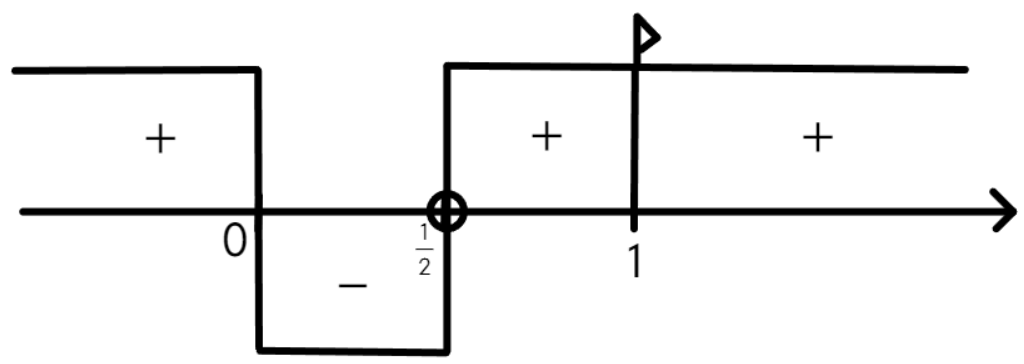
\includegraphics[scale=0.35]{ner9-60.png}}
\end{figure}\\
